\section{Versuchsaufbau}

\begin{flushleft}
    Der Versuch besteht aus den Einzelteilen: \\

    \vspace{0.3cm}

    Oszilloskop, Frequenzgenerator, RLC-Schaltung in Abbildung \ref{Abbildung4} zu sehen, Kabel, Kabel mit Tastkopf.
    
    \vspace{0.3cm}

    Der Frequenzgenerator wird über ein Kabel mit der RLC Schaltung (dem Gerät 1) verbunden.
    Die Schaltung besteht aus einer Reihenschaltung bestehend aus Spule mit Induktivität \textbf{L} und Kondensator mit Kapazität \textbf{C}. 
    In der Serienschaltung sind parallel Widerstände geschaltet. 
    Zwei davon sind fest Widerstände \textbf{R} und einer ein variabler Widerstand $\symup{\text{R}_\text{variabel}}$.

    \vspace{0.5cm}

    Der variable Widerstand wird über einen Regler am Gerät eingestellt und umfasst einen Widerstand von bis zu $10\,\unit{\kilo\ohm}$.
    Die Schaltung ist über ein Tastkopfkabel mit dem Oszilloskop verbunden. Das Signal wird auf dem Bildschirm des Oszilloskops angezeigt und kann durch verschiedene Einstellungen, verschieden Sichtbar gemacht werden.
    Der ganze Versuchsaufbau als Bild ist in Abbildung \ref{Abbildung5} gezeigt. 
\end{flushleft}

\begin{figure}[H]
    \centering
    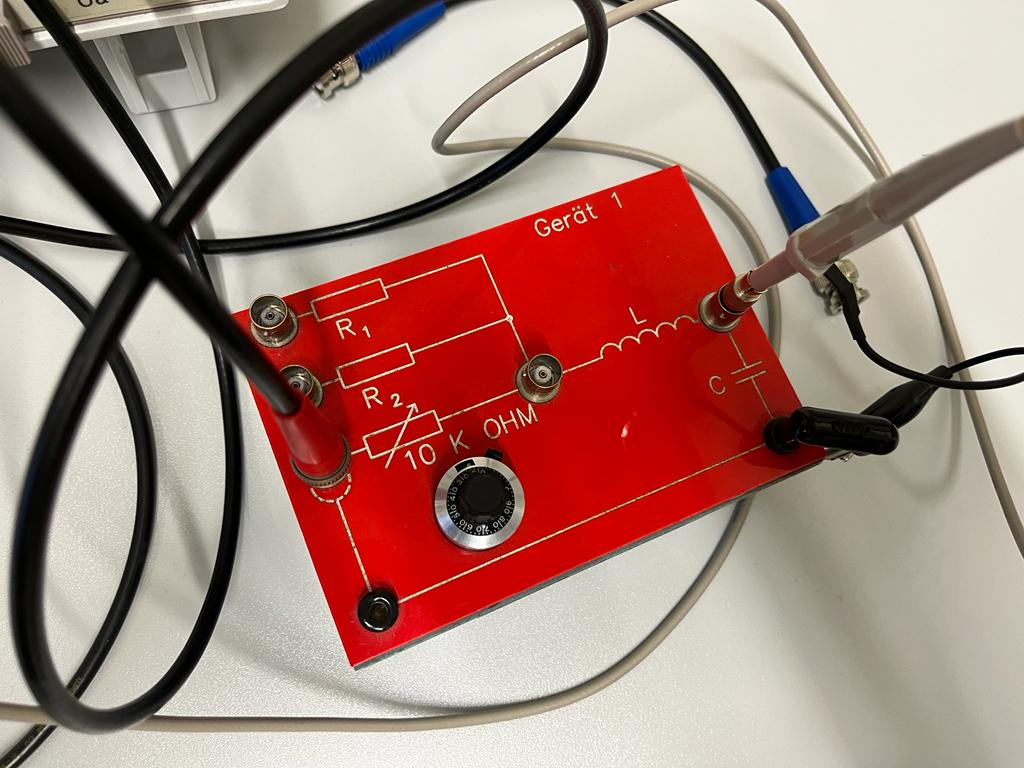
\includegraphics[width=80mm]{bilder/Ab4.jpeg}
    \caption{Ein Bild des Geräts 1 mit Tastkopf.\label{Abbildung4}}
\end{figure}

\begin{figure}[H]
    \centering
    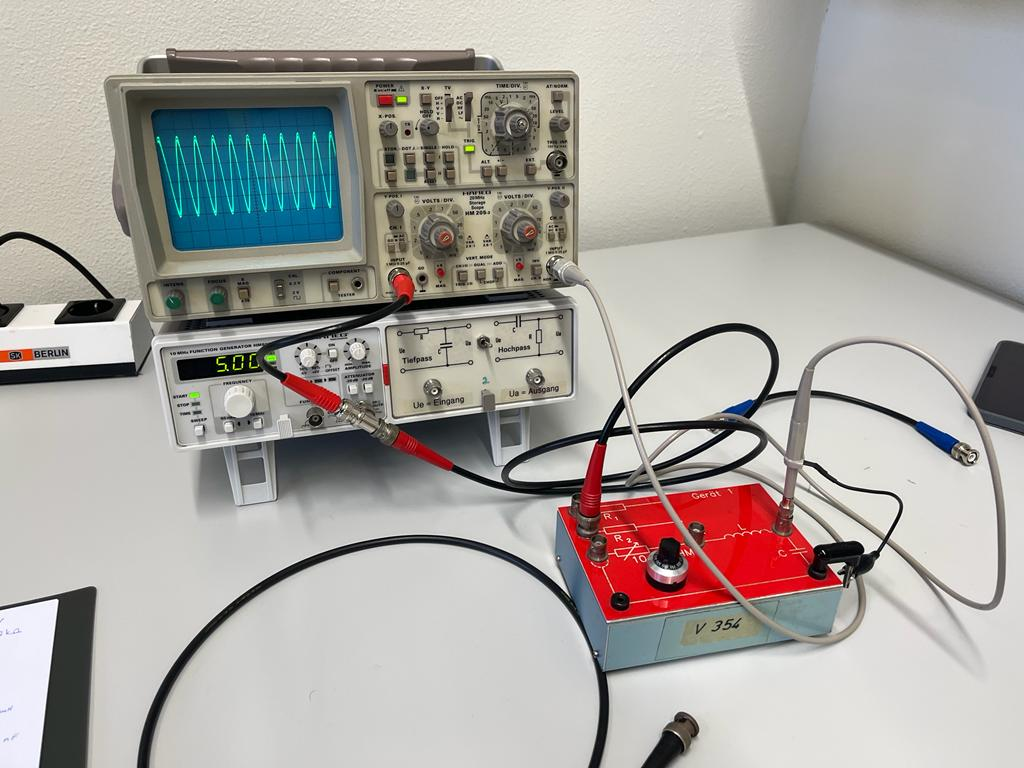
\includegraphics[width=90mm]{bilder/Ab5.jpeg}
    \caption{Übersicht auf den Kompletten Versuch (mit kleiner Erweiterung welche in Aufgabe 3 wichtig wird). \label{Abbildung5}}
\end{figure}